\documentclass{beamer}

\usepackage[utf8]{inputenc}
\usepackage[T1]{fontenc}
\usepackage{amsmath}
\usepackage{bm}

\usepackage{tabularx}
\usepackage{graphicx}
\usepackage{epstopdf}
\usepackage{multirow}

\graphicspath{{../../images/}}

\usetheme{Madrid}
\usebeamercolor{sidebartab}
\usefonttheme{professionalfonts}


\title[M.Sc. Thesis 2015]{Spatial Summarization of Image Collections}
\author{Diego A. Ballesteros Villamizar}
\institute[ETHZ]{ETH Zürich}
\date{February 8th, 2016}

\DeclareMathOperator*{\argmin}{argmin}
\DeclareMathOperator*{\argmax}{argmax}

\AtBeginSection[]
{
  \begin{frame}<beamer>
    \frametitle{Outline}
    \tableofcontents[currentsection]
  \end{frame}
}

\begin{document}

\begin{frame}
  \titlepage
\end{frame}

\section{Augmented features}

\begin{frame}{Leftover question}
  \begin{itemize}
    \item Does using a feature matrix $\mathbf{X}' = \mathbf{X} \mid \mathbb{I}$ improve the results?
    \begin{table}
      \begin{tabular}{l|lllll}
        \hline
        & \multicolumn{5}{c}{K} \\
        \hline
        \multirow{5}{*}{L} & & 0 & 2 & 5 & 10 \\
        & 0 & $17.38 \pm 1.81$ & $18.75 \pm 2.95$ & $18.82 \pm 2.58$ & $18.91 \pm 2.40$ \\
        & 2 & $22.66 \pm 4.58$ & $28.53 \pm 4.36$ &&\\
        & 5 & $25.40 \pm 4.77$ && $31.59 \pm 2.38$ &\\
        & 10 & $31.13 \pm 2.92$ &&& $30.49 \pm 3.51$ \\
      \end{tabular}
    \end{table}
    \item Not really, the best score so far is $34.35 \pm 2.15$ with $\mathbf{X} = \mathbb{I}$.
    \item Running time is significantly slower, because of the increased number of features $M = N + 4$.
  \end{itemize}
\end{frame}

\section{Sampling the distribution}

\begin{frame}{Sampling from the model}
  \begin{itemize}
    \item Using the best model, i.e. without features and with $L = 5, K=5$.
    \item How does the resulting distribution look?
    \item How to use the distribution to recommend sets?
  \end{itemize}
\end{frame}

\begin{frame}{Exact sampling}
  \begin{itemize}
    \item With $N = 10$, it is possible to calculate the probabilities from the model for all $2^{10} = 1024$ possible sets.
    \item Evaluating the model on all sets $S \subseteq V$and then normalizing the probability distribution.
    \item Takes only seconds to evaluate.
  \end{itemize}
\end{frame}

\begin{frame}{Distribution of set size ($100k$ samples)}
  \begin{figure}
    \centering
    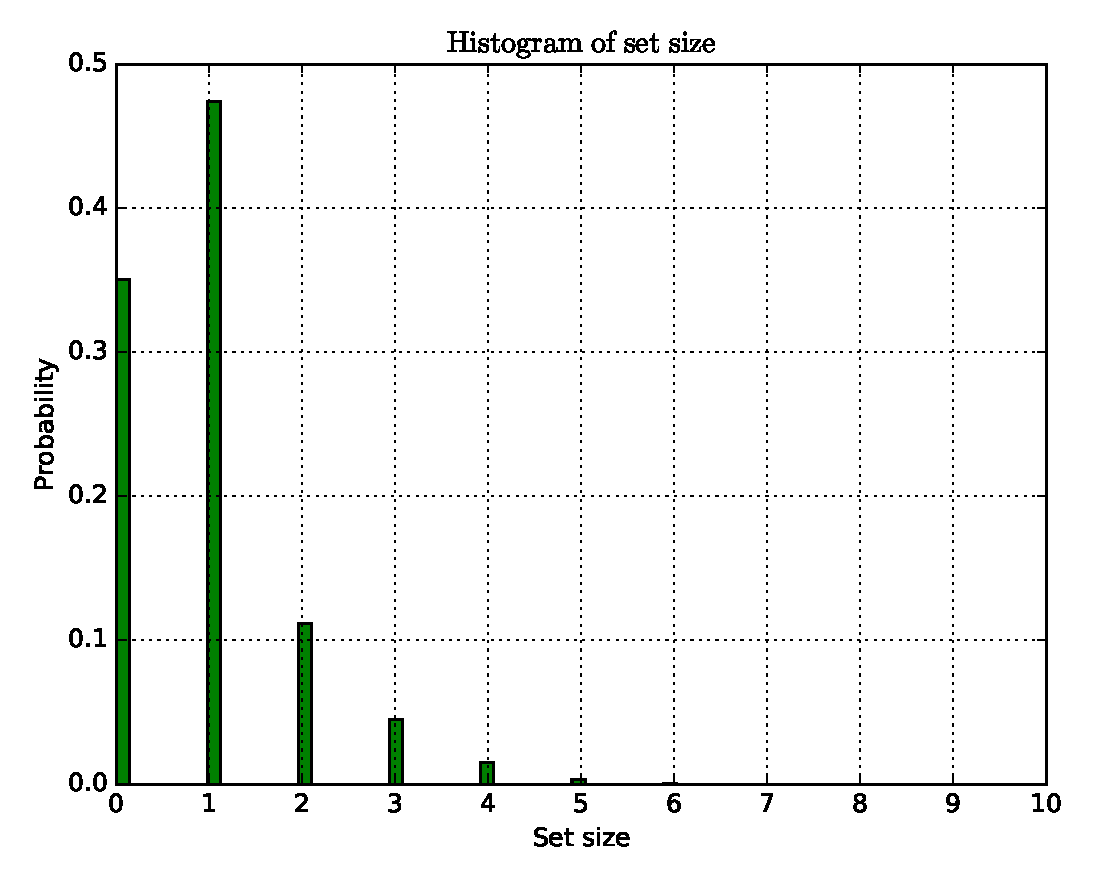
\includegraphics[height=0.8\textheight]{length_histogram_exact}
  \end{figure}
\end{frame}

\begin{frame}{Distribution of sets with $|S| = 2$ ($100k$ samples)}
  \begin{figure}
    \centering
    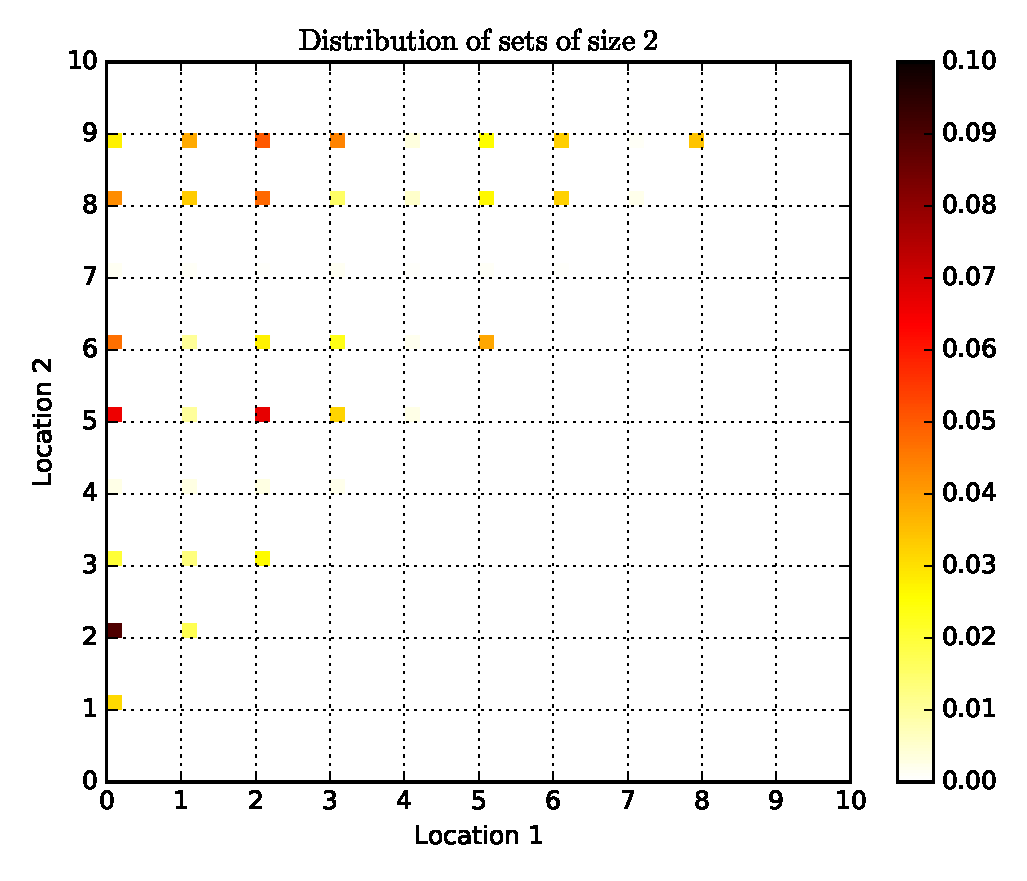
\includegraphics[height=0.8\textheight]{pairs_histogram_exact}
  \end{figure}
\end{frame}

\begin{frame}{Gibbs sampling}
  \begin{itemize}
    \item What about a method that scales? For example if $N = 30$, then there are $2^{30} = 1073741824$ sets.
    \item Gibbs sampling as presented in \cite{gotovos15sampling}.
    \item Run for $1M$ iterations, remove the first half of iterations are burn-in.
    \item Running time is a couple of minutes.
  \end{itemize}
\end{frame}

\begin{frame}{Distribution of set size ($100k$ samples)}
  \begin{figure}
    \centering
    \includegraphics[height=0.8\textheight]{length_histogram_gibbs}
  \end{figure}
\end{frame}

\begin{frame}{Distribution of sets with $|S| = 2$ ($100k$ samples)}
  \begin{figure}
    \centering
    \includegraphics[height=0.8\textheight]{pairs_histogram_gibbs}
  \end{figure}
\end{frame}

\begin{frame}{Gibbs Sampling Performance}
  \begin{figure}
    \centering
    \includegraphics[height=0.8\textheight]{gibbs_performance}
  \end{figure}
\end{frame}

\section{Extending the location set}

\begin{frame}{Use more mean-shift clusters}
  
\end{frame}

\begin{frame}{References}
  \bibliographystyle{acm}
  \bibliography{../references}
\end{frame}

\end{document}
